% ******************************* Lab report Template ***************************

\documentclass[a4paper,12pt,unnumberedsections,twoside]{Classes/LTJournalArticle}

% ******************************************************************************
% ******************************* Configurations ********************************
% ******************************************************************************

% ******************************************************************************
% Add spaces between paragraphs
%\setlength{\parskip}{0.5em}
% Ragged bottom avoids extra whitespaces between paragraphs
\raggedbottom
% To remove the excess top spacing for enumeration, list and description
%\usepackage{enumitem}
%\setlist[enumerate,itemize,description]{topsep=0em}

% *****************************************************************************
% ******************* Fonts (like different typewriter fonts etc.)*************

% *****************************************************************************
% **************************** Custom Packages ********************************

% **************************** ******Math *************************************
\usepackage{amsmath}

% ************************* Algorithms and Pseudocode **************************

%\usepackage{algpseudocode}


% ********************Captions and Hyperreferencing / URL **********************

% Captions: This makes captions of figures use a boldfaced small font.
\RequirePackage[tableposition=top]{caption}
%\DeclareCaptionFormat{custom}{#1#2\small #3}
\captionsetup{labelfont={sc,bf}, width=.9\textwidth}%format=custom, 
%\renewcommand{\figurename}{Fig.} %to support older versions of captions.sty


% *************************** Graphics and figures *****************************

%\usepackage{rotating}
%\usepackage{wrapfig}

% Uncomment the following two lines to force Latex to place the figure.
% Use [H] when including graphics. Note 'H' instead of 'h'
\usepackage{float}
%\restylefloat{figure}

% Subcaption package is also available in the sty folder you can use that by
% uncommenting the following line
% This is for people stuck with older versions of texlive
%\usepackage{sty/caption/subcaption}
\usepackage{subcaption}

% ********************************** Tables ************************************
\usepackage{booktabs} % For professional looking tables
\usepackage{multirow}
\usepackage{svg}
\usepackage{graphicx, import}

%\usepackage{multicol}
%\usepackage{longtable}
%\usepackage{tabularx}


% *********************************** SI Units *********************************
\usepackage{siunitx} % use this package module for SI units
\ifdefined\qty\else
	\ifdefined\NewCommandCopy
		\NewCommandCopy\qty\SI
	\else
		\NewDocumentCommand\qty{O{}mm}{\SI[#1]{#2}{#3}}
	\fi
	\fi
\ifdefined\unit\else
	\ifdefined\NewCommandCopy
		\NewCommandCopy\unit\si
	\else
		\NewDocumentCommand\unit{O{}m}{\si[#1]{#2}}
	\fi
\fi



% ******************************* Line Spacing *********************************

% Choose linespacing as appropriate. Default is one-half line spacing as per the
% University guidelines

% \doublespacing
% \onehalfspacing
% \singlespacing


% ************************ Formatting / Footnote *******************************

% Don't break enumeration (etc.) across pages in an ugly manner (default 10000)
%\clubpenalty=500
%\widowpenalty=500

%\usepackage[perpage]{footmisc} %Range of footnote options


% *****************************************************************************
% *************************** Bibliography  and References ********************

%\usepackage{cleveref} %Referencing without need to explicitly state fig /table

\usepackage[backend=biber]{biblatex}
% changes the default name `Bibliography` -> `References'

\usepackage{listings}
\lstdefinestyle{mystyle}{
	backgroundcolor=\color{backcolour},   
	commentstyle=\color{codegreen},
	keywordstyle=\color{magenta},
	numberstyle=\tiny\color{codegray},
	stringstyle=\color{codepurple},
	basicstyle=\ttfamily\footnotesize,
	breakatwhitespace=false,         
	breaklines=true,                 
	captionpos=b,                    
	keepspaces=true,                 
	numbers=left,                    
	numbersep=5pt,                  
	showspaces=false,                
	showstringspaces=false,
	showtabs=false,                  
	tabsize=2
}
% ******************************************************************************
% ************************* User Defined Commands ******************************
% ******************************************************************************

% *********** To change the name of Table of Contents / LOF and LOT ************

%\renewcommand{\contentsname}{My Table of Contents}
%\renewcommand{\listfigurename}{My List of Figures}
%\renewcommand{\listtablename}{My List of Tables}


% ********************** TOC depth and numbering depth *************************

\setcounter{secnumdepth}{2}
\setcounter{tocdepth}{2}


% ******************************* Nomenclature *********************************

% To change the name of the Nomenclature section, uncomment the following line

%\renewcommand{\nomname}{Symbols}


% ********************************* Appendix ***********************************

% The default value of both \appendixtocname and \appendixpagename is `Appendices'. These names can all be changed via:

%\renewcommand{\appendixtocname}{List of appendices}
%\renewcommand{\appendixname}{Appndx}

% *********************** Configure Draft Mode **********************************

% Uncomment to disable figures in `draft'
%\setkeys{Gin}{draft=true}  % set draft to false to enable figures in `draft'

% These options are active only during the draft mode
% Default text is "Draft"
%\SetDraftText{DRAFT}

% Default Watermark location is top. Location (top/bottom)
%\SetDraftWMPosition{bottom}

% Draft Version - default is v1.0
%\SetDraftVersion{v1.1}

% Draft Text grayscale value (should be between 0-black and 1-white)
% Default value is 0.75
%\SetDraftGrayScale{0.8}


% ******************************** Todo Notes **********************************
%% Uncomment the following lines to have todonotes.

%\ifsetDraft
%	\usepackage[colorinlistoftodos]{todonotes}
%	\newcommand{\mynote}[1]{\todo[author=kks32,size=\small,inline,color=green!40]{#1}}
%\else
%	\newcommand{\mynote}[1]{}
%	\newcommand{\listoftodos}{}
%\fi

% Example todo: \mynote{Hey! I have a note}


\addbibresource{References/references.bib}

%\runninghead{} % A shortened article title to appear in the running head, leave this command empty for no running head

%\footertext{\textit{} % Text to appear in the footer, leave this command empty for no footer text

\setcounter{page}{1} % The page number of the first page, set this to a higher number if the article is to be part of an issue or larger work

\title{Electroosmotic Flow and Electrophoresis} % Article title, use manual lines breaks (\\) to beautify the layout

\author{%
	Niklas Scheuler, Niklas Müller and Jonas Scheunemann
}

\renewcommand{\maketitlehookd}{%
	\begin{abstract}
		\noindent Empty abstract.
	\end{abstract}
}


\begin{document}


\maketitle

% *********************** Adding TOC  ***********************

\tableofcontents

% \printnomenclature[space] space can be set as 2em between symbol and description
%\printnomenclature[3em]

% ******************************** Main Matter *********************************

%%!TEX root = ../Lab_report.tex
%*******************************************************************************
%*********************************** Theory Chapter *****************************
%*******************************************************************************
\section{Theory}
\subsection{Lattice-Boltzmann method}
The Boltzmann equation describes the statistical behavior of a thermodynamic system out of equilibrium. It is given by:

\begin{equation}\label{eq:boltzmann-transport}
\frac{\partial f}{\partial t} + \mathbf{v} \cdot \nabla_{\mathbf{r}} f + \mathbf{F} \cdot \nabla_{\mathbf{v}} f = \left( \frac{\partial f}{\partial t} \right)_{\text{coll}}
\end{equation}

where \( f = f(\mathbf{r}, \mathbf{v}, t) \) is the distribution function, \( \mathbf{r} \) is the position, \( \mathbf{v} \) is the velocity, \( \mathbf{F} \) is the external force and \( \left( \frac{\partial f}{\partial t} \right)_{\text{coll}} \) is the collision term.

The Bhatnagar-Gross-Krook (BGK) approximation simplifies the collision term to 

\begin{equation}\label{eq:collision}
\left( \frac{\partial f}{\partial t} \right)_{\text{coll}} = -\frac{1}{\tau} (f - f^{\text{eq}})
\end{equation}
where \( \tau \) is the relaxation time and \( f^{\text{eq}} \) is the local equilibrium distribution function. We assume that there is a equilibrium distribution to which the system relaxes. How fast this equilibrium is reached is encoded in the relaxation time $\tau$, which corresponds directly to the viscosity of the fluid.\\

The Ansatz for the Lattice Boltzmann Method (LBM) is now to discretise the position space and form a lattice as well as discretising the time. The distributions are then also discretised, with each lattice site having the number of distributions corresponding to neighbouring sites. This number of neighbours depends on the lattice model used. So for each time step the collision is calculated with \autoref{eq:collision} for each of the different distributions $f_i$ on a single lattice site. Then the streaming to the other lattice sites is calculated using the final form of the approximation of \autoref{eq:boltzmann-transport}

\begin{equation}
f_i(\mathbf{r} + \mathbf{e}_i \Delta t, t + \Delta t) = f_i(\mathbf{r}, t) + \frac{\Delta t}{\tau} \left( f_i^{\text{eq}}(\mathbf{r}, t) - f_i(\mathbf{r}, t) \right)
\end{equation}

Advantages of the LBM are the high parralisability of the computations, resulting in short simulation times, and the efficient simulation of multi-phase fluids.
Disadvantages are the high memory consumption and the fact that LBM can't calculate fluids with a high Mach number meaning compressible flows.



\subsection{Particle-Particle - Particle-Mesh}

The P3M algorithm, also known as the Particle-Particle Particle-Mesh method, is a computational approach utilized for efficient computation of long-range interactions in systems with periodic boundary conditions. This method is particularly useful in molecular dynamics simulations.

\subsubsection{Ewald summation}
Ewald summation is a technique used to compute non-neglectable long-range interactions in periodic systems by splitting the potential into short-range and long-range components. Looking at a charge distribution of a Coulomb potential with 
\begin{equation}
\rho = \sum_{\mathbf{n} \in \mathbb{L}^3} \sum_{i=1}^{N} q_i \delta(\mathbf{r} - \mathbf{r}_i - \mathbf{n})
\end{equation}
we can add a gaussian shielding charge of the form
$ \rho_{\text{Gauss}}(\mathbf{r}) = \left( \frac{\alpha}{\sqrt{\pi}} \right)^3 e^{-\alpha^2 r^2}$ 
for each charged particle  with a width $a$, turning the delta function into
\begin{equation}
\delta(\mathbf{r}) = \rho_{\text{Gauss}}(\mathbf{r})+ {[\delta(\mathbf{r}) - \rho_{\text{Gauss}}(\mathbf{r})]}.
\end{equation}

The potential for the Coulomb Ewald Summation can now be written with a real space, k-space and a self-interaction part
\begin{equation}
  U = U^{r} + U^{k} + U^{s}
\end{equation}

\begin{align*}
  U^{r} &= \frac{l_B}{2} \sum_{\mathbf{m} \in \mathbb{Z}^3} \sum_{i,j}' \frac{q_i q_j \, \text{erfc}(\alpha | \mathbf{r}_{ij} + \mathbf{m}L |)}{| \mathbf{r}_{ij} + \mathbf{m}L |}  \\
  U^{k} &= \frac{l_B}{2L^3} \sum_{\mathbf{k} \neq 0} \frac{4\pi}{k^2} e^{-k^2 / 4\alpha^2} |\hat{\rho}(\mathbf{k})|^2 \\
  U^{s} &= -\frac{\alpha l_B}{\sqrt{\pi}} \sum_{i} q_i^2\\
\end{align*}

\subsubsection{P3M algorithm steps}
The idea of the P3M algorithm is now to speed up the reciprocal space calculations by calculating them on a grid.
So for the first step we need to transform the charges onto a mesh. 
This is done with 
\begin{equation}
  \rho_M(\mathbf{r}_p) = \frac{1}{h^3} \sum_{i=1}^{N} q_i W^{p}(\mathbf{r}_p - \mathbf{r}_i)
\end{equation}
where $W^{p}(\mathbf{r}_p - \mathbf{r}_i)$ are cardinal B-Splines.
With the mesh initialized we need ot obtain the fourier transformed charge distribution $\hat{\rho}(k)$, so we can solve the Poisson equation with
\begin{equation}
  \hat{\phi}(k) = G(k)\hat{\rho}(k)
\end{equation}
where $G(k)$ is the optimal influence function.
With this it is only a matter of obtaining the field by differentiation in Fourier space $ik\hat{\phi}(k) = \hat{E}(k)$, transforming back to real space  and interpolating the field at position of charges to get the forces for the MD calculations. 

%%!TEX root = ../Lab_report.tex
%*******************************************************************************
%*********************************** Methods Chapter *****************************
%*******************************************************************************
\section{Methods}

%********************************** %First Section  **************************************



%!TEX root = ../Lab_report.tex
%*******************************************************************************
%*********************************** Analysis Chapter *****************************
%*******************************************************************************
\section{Free-Solution DNA electrophoresis}
Electrophoresis is an experimental technique used to separate charged molecules like polyelectrolyte chains by making use of the interaction between the particles and external electric fields. In a solution with counterions, the dynamics of a charged polymer chain is governed by electrostatic interactions between polymers and counterions as well as hydrodynamic interactions. We investigate the dynamical properties of polyelectrolytes of different lengths in a bulk solution using coarse grained Molecular Dynamics simulations with electrostatics and hydrodynamical interactions. All simulations were carried out with ESPResSo \cite{weik2019espresso}. Electrostatic interactions are modelled efficiently with the P3M method with periodic boundary conditions. The Lattice-Boltzmann method (LBM) is employed to model hydrodynamical interactions.

\subsection{System setup}
We conducted several simulations of a system with equal parameters except the number of monomers $N$ on the polyelectrolyte chain. In every simulation the system consisted of $N$ (where $1\le N \ge 32$)monomers connected by bonded interactions modelled with a FENE potential. Furthermore, $N$ counterions are placed at random positions in the simulation box. All simulated particles exhibited short ranged repulsive interactions, modelled by a WCA potential and long ranged electrostatic interactions, where a Bjerrum length of $l_\text{B} = 2.84$ in reduced units was chosen. The box size of the cubic simulation box was chosen such that the mean concentration of monomers in the solution was kept constant at $\SI{5}{\milli M}$. To remove overlap between all particles in the system, first, a total of $2000$ gradient based energy minimization steps were performed to remove overlap between all particles in the system. Subsequently, after activating electrostatic and hydrodynamic interactions, the system was equilibrated for $\SI{5e5}{}$ integration steps. During the production run, we sampled data every integration step for a total of $\SI{5e6}{}$ steps. Figure \ref{fig:vmd} displays the simulated system for one simulation with $N=32$ after equilibration.
\begin{figure}[H]
	\centering
	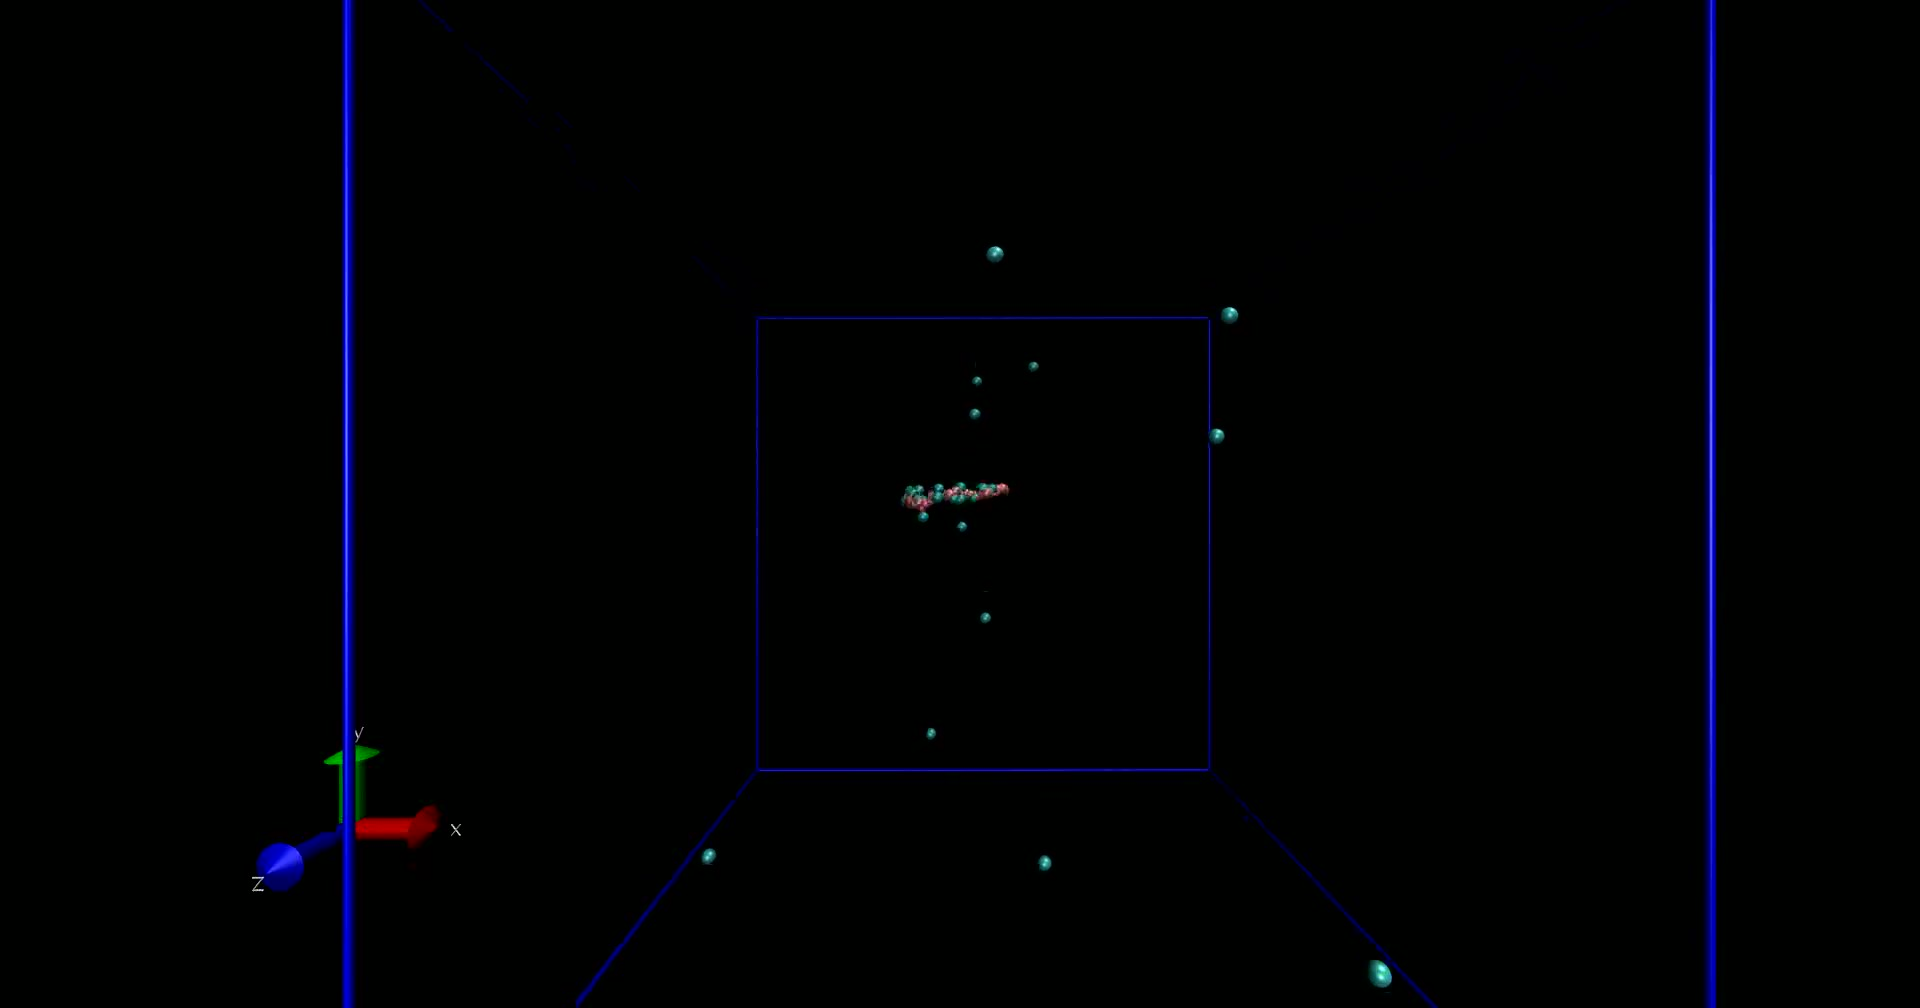
\includegraphics[width=\columnwidth]{Analysis_1/VMD_visualization}
	\captionsetup{width=\columnwidth}
	\caption{Visualization of a simulated polyelectrolyte with a chain length of 32.}
	\label{fig:vmd}
\end{figure}
%%!TEX root = ../Lab_report.tex
%*******************************************************************************
%*********************************** Additional sections for analysis Chapter *****************************
%*******************************************************************************

\section{Electro-Osmotic flow}
Electro-Osmotic flow plays a crucial role in various scientific and industrial processes, especially in microfluidics, electrochemistry, and environmental science. In this work, the electro-osmotic flow of ions in a solution within a charged slit pore is investigated. We take a closer look at the density distribution of the ions as well as the flow profile of the solvent.
\subsection{System setup}
A snapshot of the system is shown in Figure \ref{fig:system1}. It consists of two infinite, parallel, charged walls with ions and a solvent in between. The ions are accelerated by an electric field.  In order to reduce the degrees of freedom, the solvent is represented by an Lattice-Boltzmann Fluid. The wall charge is represented by 64 charged particles with the charge $q=\text{e}$ that are fixed on each wall. They create an electric field that is homogeneous enough for our application. To keep the system electrically neutral, 128 counter ions are placed between the walls. Periodic boundary conditions are used in the plane  parallel to the walls.  The electrostatic interactions are solved by the ELC algorithm. Additionally all particles interact with each other and the walls via the Weeks-Chandler-Andersen potential. The simulation is performed with ESPResSo. A list with the system parameters can be found in the Appendix in Table \ref{tab:params}.
The python code can also be found in the Appendix. In the production runs, the simulations were always executed for 100000 integration steps and a step size $\Delta t= 0.01\,[t]$. Since the sampling of the flow and the density profile is numerically costly, only  every hundredth data point of the flow and the density profile was sampled.
\begin{figure}[H]
	\centering
	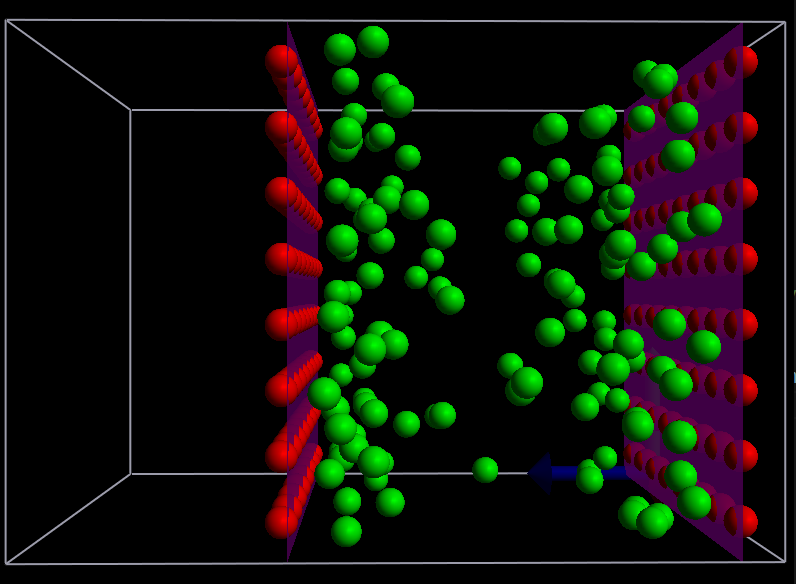
\includegraphics[width=\columnwidth]{Analysis_2/system}
	\captionsetup{width=\columnwidth}
	\caption{Visualization of the slit pore system. The wall charges (counter ions) are represented by red (green) spheres. The ELC gap is clearly visible on the left hand side of the left hand wall.}
	\label{fig:system}
\end{figure}
\subsection{Results}
The flow profile of the solvent is a characteristic observable of a system with electro-osmotic flow. As explained in section \ref{ } it can be calculated analytically in the continuum limit. The analytical solution yields a flat profile. This profile is highest at the center and goes to zero at the boundary. Figure \ref{fig:slit_plot} shows the flow profile obtained by the simulation as well as the theoretical curve. It can be seen that there is a good agreement.

\begin{figure}[H]
	\centering
	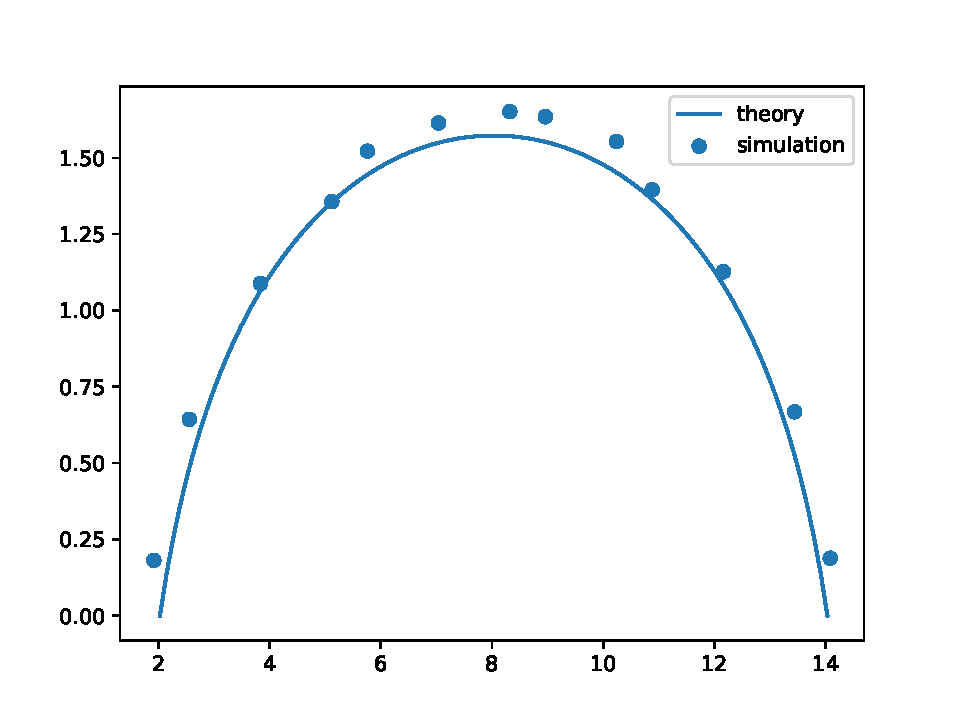
\includegraphics[width=\columnwidth]{slit_pore/prodrun_figs/fp}
	\captionsetup{width=\columnwidth}
	\caption{Comparison of the simulation data and the theoretical calculations of the flow profile.}
	\label{fig:slit_plot}
\end{figure}

Another interesting observable is the ion density profile. It can also be calculated in the continuum limit. Due to the opposing charge of the wall and the ions, they attract each other. Therefore, the ions accumulate close to the boundary. Due to the repulsion between  the ions, not all of the ions condensate at the wall. This behavior can be seen in Figure \ref{fig:slit_plot2}
\begin{figure}[H]
	\centering
	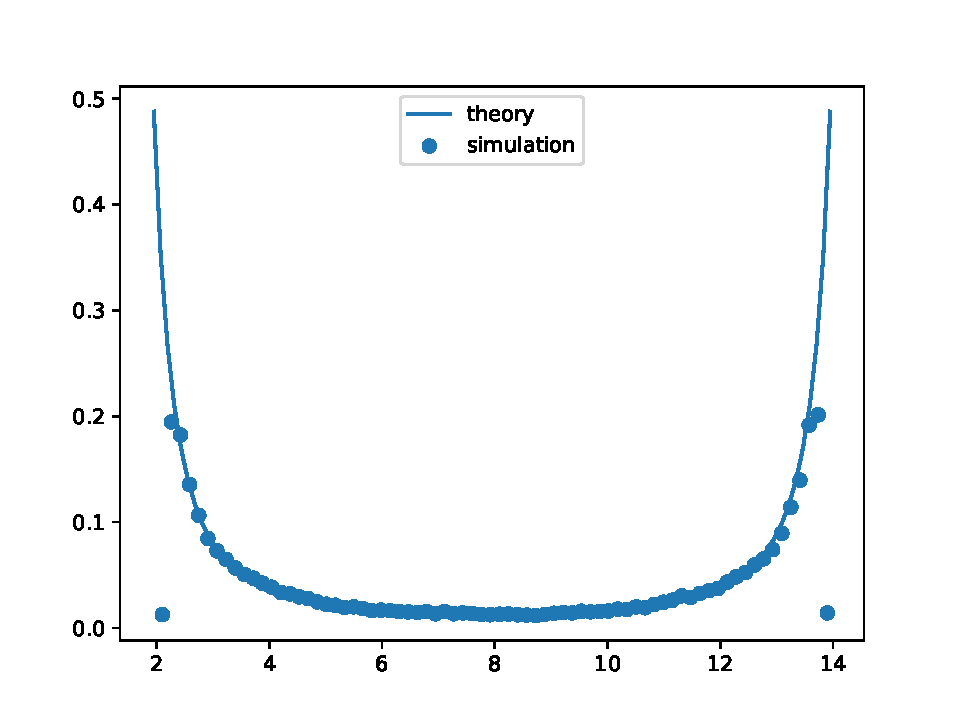
\includegraphics[width=\columnwidth]{slit_pore/prodrun_figs/id}
	\captionsetup{width=\columnwidth}
	\caption{Comparison of the simulation data and the theoretical calculations of the ion density.}
	\label{fig:slit_plot2}
\end{figure}
\begin{table}[H]
	\caption{System parameter in SI units and simulation units}
	\centering
	\begin{tabular}{l c c c c c}
		\toprule
		parameter  & value (SI units) & value (simulation units)\\
		\midrule
		channel width $d$&\SI{12}{nm}&12[x]\\
		counter ion charge $q$&\SI{1}{e}&1[q]\\
		thermal energy $k_{\text{B}}T$&$k_{\text{B}}\SI{300}{K}$&1[E]\\
		vacuum permittivity $\varepsilon_\text{0}$&\SI{8.85e-10}{s^2kgm^3}&\SI{1.428e-3}{}$[q]^2[t]^2/[m][x]^3$\\
		relative solvent permittivity5  $\varepsilon_\text{r}$&\SI{78.54}{}&78.54\\
		external electrical field $E$&\SI{0.646e9}{Vm^{-1}}&$25[E]/[q][x]$\\
		solvent density $\rho$&\SI{1000}{kg\per m^3}&$26.18[m]/[x]^3$\\
		kinematic solvent viscosity $\nu$&\SI{8.23e-8}{m^2\per s}&$0.25[x]^2/[t]$\\
		counterion frictional coefficient $\gamma$&\SI{1.910}{kg\per s}&15[m]/[t]\\
		\bottomrule
	\end{tabular}	
	\label{tab:params}
\end{table}

%%!TEX root = ../Lab_report.tex
%*******************************************************************************
%*********************************** First Chapter *****************************
%*******************************************************************************

\chapter{Results}  %Title of the Third Chapter

%********************************** %First Section  **************************************

%%!TEX root = ../Lab_report.tex
% ******************************* Thesis Appendix A ****************************
\chapter{How to install \LaTeX} 

\section*{Windows OS}

\subsection*{TeXLive package - full version}
\begin{enumerate}
\item	Download the TeXLive ISO (2.2GB) from\\
\href{https://www.tug.org/texlive/}{https://www.tug.org/texlive/}
\item	Download WinCDEmu (if you don't have a virtual drive) from \\
\href{http://wincdemu.sysprogs.org/download/}
{http://wincdemu.sysprogs.org/download/}
\item	To install Windows CD Emulator follow the instructions at\\
\href{http://wincdemu.sysprogs.org/tutorials/install/}
{http://wincdemu.sysprogs.org/tutorials/install/}
\item	Right click the iso and mount it using the WinCDEmu as shown in \\
\href{http://wincdemu.sysprogs.org/tutorials/mount/}{
http://wincdemu.sysprogs.org/tutorials/mount/}
\item	Open your virtual drive and run setup.pl
\end{enumerate}

or

\subsection*{Basic MikTeX - \TeX~ distribution}
\begin{enumerate}
\item	Download Basic-MiK\TeX (32bit or 64bit) from\\
\href{http://miktex.org/download}{http://miktex.org/download}
\item	Run the installer 
\item	To add a new package go to Start >> All Programs >> MikTex >> Maintenance (Admin) and choose Package Manager
\item	Select or search for packages to install
\end{enumerate}

\subsection*{TexStudio - \TeX~ editor}
\begin{enumerate}
\item	Download TexStudio from\\
\href{http://texstudio.sourceforge.net/\#downloads}
{http://texstudio.sourceforge.net/\#downloads} 
\item	Run the installer
\end{enumerate}

\section*{Mac OS X}
\subsection*{MacTeX - \TeX~ distribution}
\begin{enumerate}
\item	Download the file from\\
\href{https://www.tug.org/mactex/}{https://www.tug.org/mactex/}
\item	Extract and double click to run the installer. It does the entire configuration, sit back and relax.
\end{enumerate}

\subsection*{TexStudio - \TeX~ editor}
\begin{enumerate}
\item	Download TexStudio from\\
\href{http://texstudio.sourceforge.net/\#downloads}
{http://texstudio.sourceforge.net/\#downloads} 
\item	Extract and Start
\end{enumerate}


\section*{Unix/Linux}
\subsection*{TeXLive - \TeX~ distribution}
\subsubsection*{Getting the distribution:}
\begin{enumerate}
\item	TexLive can be downloaded from\\
\href{http://www.tug.org/texlive/acquire-netinstall.html}
{http://www.tug.org/texlive/acquire-netinstall.html}.
\item	TexLive is provided by most operating system you can use (rpm,apt-get or yum) to get TexLive distributions
\end{enumerate}

\subsubsection*{Installation}
\begin{enumerate}
\item	Mount the ISO file in the mnt directory
\begin{verbatim}
mount -t iso9660 -o ro,loop,noauto /your/texlive####.iso /mnt
\end{verbatim}

\item	Install wget on your OS (use rpm, apt-get or yum install)
\item	Run the installer script install-tl.
\begin{verbatim}
	cd /your/download/directory
	./install-tl
\end{verbatim}
\item	Enter command `i' for installation

\item	Post-Installation configuration:\\
\href{http://www.tug.org/texlive/doc/texlive-en/texlive-en.html\#x1-320003.4.1}
{http://www.tug.org/texlive/doc/texlive-en/texlive-en.html\#x1-320003.4.1} 
\item	Set the path for the directory of TexLive binaries in your .bashrc file
\end{enumerate}

\subsubsection*{For 32bit OS}
For Bourne-compatible shells such as bash, and using Intel x86 GNU/Linux and a default directory setup as an example, the file to edit might be \begin{verbatim}
edit $~/.bashrc file and add following lines
PATH=/usr/local/texlive/2011/bin/i386-linux:$PATH; 
export PATH 
MANPATH=/usr/local/texlive/2011/texmf/doc/man:$MANPATH;
export MANPATH 
INFOPATH=/usr/local/texlive/2011/texmf/doc/info:$INFOPATH;
export INFOPATH
\end{verbatim}
\subsubsection*{For 64bit OS}
\begin{verbatim}
edit $~/.bashrc file and add following lines
PATH=/usr/local/texlive/2011/bin/x86_64-linux:$PATH;
export PATH 
MANPATH=/usr/local/texlive/2011/texmf/doc/man:$MANPATH;
export MANPATH 
INFOPATH=/usr/local/texlive/2011/texmf/doc/info:$INFOPATH;
export INFOPATH

\end{verbatim}



%\subsection{Installing directly using Linux packages} 
\subsubsection*{Fedora/RedHat/CentOS:}
\begin{verbatim} 
sudo yum install texlive 
sudo yum install psutils 
\end{verbatim}


\subsubsection*{SUSE:}
\begin{verbatim}
sudo zypper install texlive
\end{verbatim}


\subsubsection*{Debian/Ubuntu:}
\begin{verbatim} 
sudo apt-get install texlive texlive-latex-extra 
sudo apt-get install psutils
\end{verbatim}


% ********************************** Bibliography ******************************

\printbibliography % Output the bibliography

\end{document}
